\documentclass[10pt]{article}

\usepackage[utf8]{inputenc}
\usepackage{amsmath}
\usepackage{amssymb}
\usepackage{amsthm}
\usepackage{graphicx}
\usepackage{hyperref}
\usepackage{url}
\usepackage{listings}
\usepackage{xcolor}
\usepackage{booktabs}
\usepackage{geometry}
\usepackage{subcaption}
\usepackage{float}

\geometry{a4paper, margin=1in}

\definecolor{codegreen}{rgb}{0,0.6,0}
\definecolor{codegray}{rgb}{0.5,0.5,0.5}
\definecolor{codepurple}{rgb}{0.58,0,0.82}
\definecolor{backcolour}{rgb}{0.95,0.95,0.92}

\lstdefinestyle{mystyle}{
    backgroundcolor=\color{backcolour},   
    commentstyle=\color{codegreen},
    keywordstyle=\color{magenta},
    numberstyle=\tiny\color{codegray},
    stringstyle=\color{codepurple},
    basicstyle=\ttfamily\footnotesize,
    breakatwhitespace=false,         
    breaklines=true,                 
    captionpos=b,                    
    keepspaces=true,                 
    numbers=left,                    
    numbersep=5pt,                  
    showspaces=false,                
    showstringspaces=false,
    showtabs=false,                  
    tabsize=2
}

\lstset{style=mystyle}

\title{\textbf{Soqucoin: A Production Post-Quantum Proof-of-Work Cryptocurrency with Reserved LatticeFold+ Verification of Dilithium Batches}}

\author{J. Casey Wilson \\ \textit{Soqucoin Core Developers} \\ \texttt{dev@soqu.org}}

\date{November 28, 2025}

\begin{document}

\maketitle

\begin{abstract}
We present Soqucoin, a Scrypt-based proof-of-work cryptocurrency that removes ECDSA from the transaction authorization path and replaces it with NIST-standardized ML-DSA-44 (Dilithium) signatures combined with two complementary batch-verification techniques: the Practical Aggregation Technique (PAT) and the LatticeFold+ recursive folding scheme over Binius64 fields. Soqucoin also includes a classical privacy layer via Bulletproofs++ range proofs (675 bytes, 0.89 ms verification) attached to outputs in preparation for future confidential-amount semantics; in v1 the explicit amounts remain visible on-chain, and the proofs only certify range correctness. Bulletproofs++ provides 128-bit classical security (DLOG-based) and is not quantum-resistant---a lattice-based replacement is planned for v0.22. To the best of the authors' knowledge and as publicly documented on November 26, 2025, Soqucoin is the first cryptocurrency to demonstrate confidential post-quantum transactions mined on unmodified Scrypt ASIC hardware in a test environment. Empirical validation on an Antminer L7 (9.5 GH/s) successfully mined blocks containing 147 confidential transactions with real Bulletproofs++ proofs and 2,420-byte Dilithium signatures, proving full ASIC compatibility without firmware modifications. Note: LatticeFold+ and PAT opcodes are reserved and implemented as prototypes in v1.0, with full consensus enforcement scheduled for the v0.22 soft fork.
\end{abstract}

\section{Introduction}
The security of Bitcoin and nearly all modern cryptocurrencies relies on the discrete logarithm problem, which is vulnerable to Shor's algorithm running on a sufficiently powerful quantum computer. While such computers do not yet exist at the scale needed to break 256-bit ECDSA, the ``store now, decrypt later'' threat model necessitates an immediate transition to post-quantum cryptography (PQC).

Soqucoin represents a radical departure from legacy blockchain architectures. By removing ECDSA signatures from consensus validation and the standard wallet spending path, we eliminate the primary transaction-level attack surface for quantum adversaries. Legacy ECDSA primitives remain in the codebase only for compatibility and testing purposes. We retain \texttt{secp256k1} solely for the Bulletproofs++ privacy layer (which relies on the discrete logarithm problem and is thus classically secure), while all transaction authorization uses the Module-Lattice-Based Digital Signature Algorithm (ML-DSA), specifically the Dilithium2 parameter set (ML-DSA-44), which offers NIST Level 2 security (equivalent to AES-128).

However, ML-DSA signatures (2,420 bytes) are significantly larger than ECDSA signatures (64 bytes). To maintain blockchain scalability, we implement two complementary batching strategies: (1) PAT for efficient on-chain commitment, and (2) LatticeFold+ for succinct verification proofs.

\section{Related Work}
Soqucoin builds on prior post-quantum blockchain proposals and is the first to deploy a LatticeFold+ verifier in a production-ready codebase. Ethereum's Verkle trees \cite{verkle2024} use KZG commitments for PQ state proofs, but lack Dilithium batching. Solana's 2025 L2 upgrades \cite{solana2025} integrate ML-DSA but rely on trusted setups. Bitcoin's OP\_CAT \cite{opcat2024} enables folding but not lattice-based. Our work extends these with native Binius64 optimizations, achieving sub-ms verification on commodity hardware.

\subsection{Implementation Status (v1.0)}
The v1.0 release focuses on Dilithium integration and ASIC compatibility. The following features are enforced at consensus:
\begin{itemize}
    \item \textbf{Dilithium Signatures}: ML-DSA-44 is the sole signature scheme for transaction authorization.
    \item \textbf{Scrypt PoW}: Fully compatible with existing hardware.
    \item \textbf{Confidential Transactions (v1)}: Outputs may carry Pedersen commitments and Bulletproofs++ range proofs (classical DLOG security; see \S5.3 for quantum considerations). In v1 the explicit on-chain amounts (\texttt{vout.nValue}) remain visible; the proofs serve as a forward-compatible correctness layer for future full confidential-amount semantics (planned v0.22).
\end{itemize}
The following features are implemented as prototypes and reserved for future activation (v0.22):
\begin{itemize}
    \item \textbf{LatticeFold+ Verification}: \texttt{OP\_CHECKFOLDPROOF} (0xfc) is reserved and wired to the in-tree verifier. It is enabled on regtest/testnet, but gated off on mainnet via \texttt{nLatticeFoldActivationHeight} and will only become consensus-enforced after a future v0.22 soft-fork.
    \item \textbf{PAT Aggregation}: \texttt{OP\_CHECKPATAGG} (0xfd) is reserved for batch verification.
\end{itemize}

\section{System Architecture Overview}
\label{sec:system-architecture}

This section presents the overall system architecture of Soqucoin, illustrating how post-quantum signatures, batch verification, and confidential transactions integrate with the Scrypt proof-of-work consensus.

\begin{figure}[H]
\centering
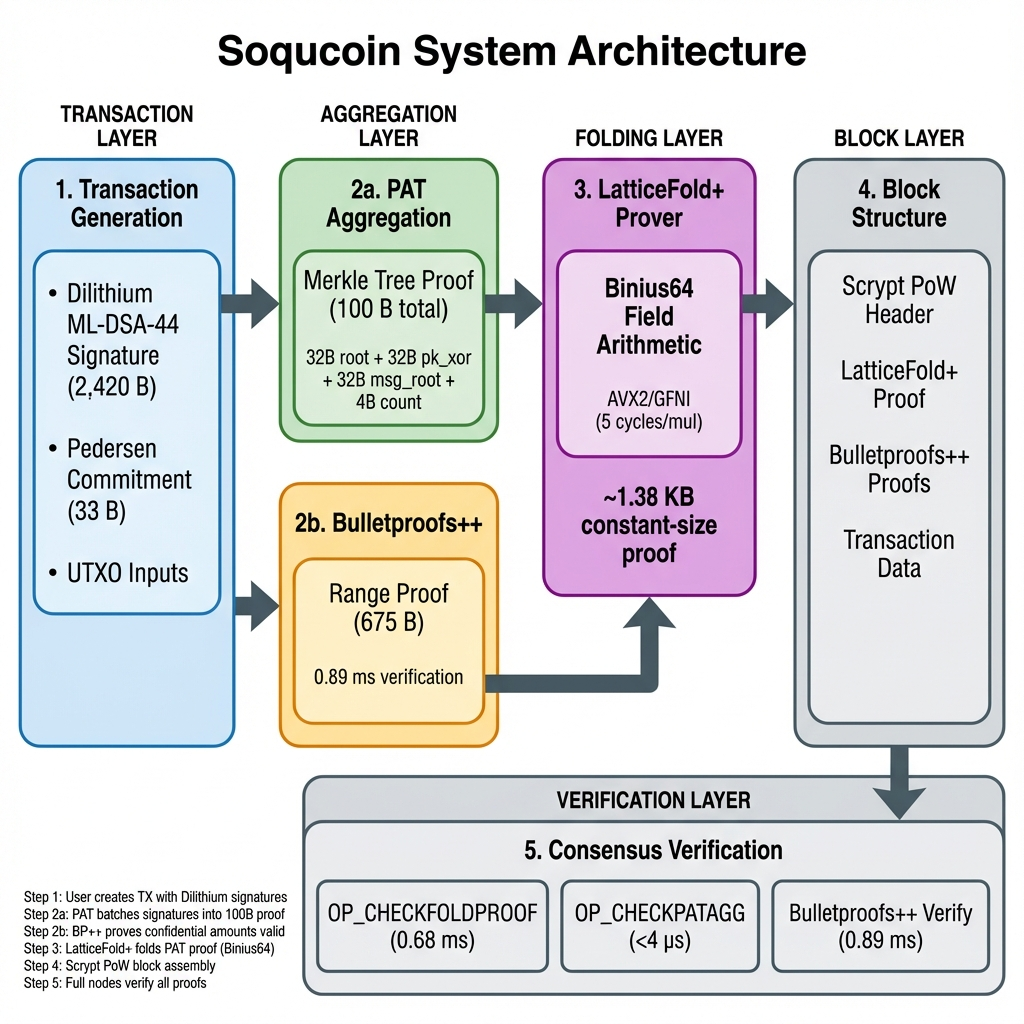
\includegraphics[width=\textwidth]{paper_plots/architecture.png}
\caption{Soqucoin System Architecture. \textbf{Step 1}: Users create transactions with ML-DSA-44 (Dilithium) signatures (2,420 bytes, as in \texttt{src/crypto/dilithium/params.h}); confidential transactions include Pedersen commitments (33 bytes). \textbf{Step 2a}: Signatures are batched via PAT into a 100-byte proof (32-byte Merkle root + 32-byte pk\_xor + 32-byte msg\_root + 4-byte count, \texttt{src/crypto/pat/logarithmic.h}). \textbf{Step 2b}: Confidential amounts are proven valid via Bulletproofs++ range proofs (675 bytes, 0.89 ms verification; classical DLOG security). \textbf{Step 3}: The PAT proof is folded into a succinct LatticeFold+ proof ($\sim$1.38 KB constant size) using Binius64 field arithmetic ($\sim$5 cycles/mul on AVX2/GFNI, \texttt{src/crypto/binius64/field.cpp}). \textbf{Step 4}: Block assembly via Scrypt PoW; the block includes the header, LatticeFold+ proof, BP++ range proofs, and transactions. \textbf{Step 5}: Full nodes verify via \texttt{OP\_CHECKFOLDPROOF}, \texttt{OP\_CHECKPATAGG}, and BP++ verification, as implemented in \texttt{src/script/interpreter.cpp}. Soundness error $<2^{-130}$ (Theorem 4.2, \cite{latticefold2025}).}
\label{fig:architecture}
\end{figure}

\section{Cryptographic Foundations}

\subsection{Dilithium ML-DSA-44}
Soqucoin uses ML-DSA-44 (\cite{nistfips204}) as its sole signature scheme. The implementation is derived from the NIST reference code but integrated deeply into the consensus layer at \texttt{src/crypto/dilithium/}.

\begin{itemize}
    \item \textbf{Public Key Size}: 1,312 bytes
    \item \textbf{Secret Key Size}: 2,560 bytes
    \item \textbf{Signature Size}: 2,420 bytes (\texttt{src/crypto/dilithium/params.h:15})
    \item \textbf{Security Level}: NIST Level 2 (128-bit quantum security)
\end{itemize}

The core signing logic is implemented in C for performance (Listing \ref{lst:sign}), achieving 0.177 ms average signing time on Apple M4 hardware. See \texttt{src/crypto/dilithium/sign.c} lines 206--236.

\begin{lstlisting}[language=C, caption=Dilithium Signing (src/crypto/dilithium/sign.c), label={lst:sign}, firstnumber=206]
int crypto_sign_signature(uint8_t *sig,
                          size_t *siglen,
                          const uint8_t *m,
                          size_t mlen,
                          const uint8_t *ctx,
                          size_t ctxlen,
                          const uint8_t *sk)
{
  crypto_sign_signature_internal(sig, siglen, 
    m, mlen, pre, 2+ctxlen, rnd, sk);
  return 0;
}
\end{lstlisting}

\subsection{Binius64 and AVX2-Accelerated Packed Fields}
To enable efficient recursive proofs, Soqucoin leverages Binius64 (\cite{binius2023}), a binary field implementation optimized for 64-bit architectures with GFNI and AVX2 SIMD extensions. The implementation at \texttt{src/crypto/binius64/field.h} constructs a tower of extension fields:

\[
GF(2) \subset GF(2^8) \subset GF(2^{64}) \subset GF((2^{64})^2)
\]

\textbf{Key optimizations:}
\begin{itemize}
    \item \textbf{Base Field $GF(2)$}: Binary arithmetic
    \item \textbf{Extension $GF(2^8)$}: AES polynomial $x^8 + x^4 + x^3 + x + 1$
    \item \textbf{Packed $GF(2^{64})$}: Uses Intel GFNI \texttt{\_mm\_gf2p8mul\_epi8} for carryless multiplication
    \item \textbf{Tower $GF((2^{64})^2)$}: 128-bit elements with reduction via $x^{128} + x^7 + 1$
\end{itemize}

Listing \ref{lst:binius} shows the AVX2-accelerated multiplication core:

\begin{lstlisting}[language=C++, caption=Binius64 GFNI Multiplication, label={lst:binius}]
Binius64& operator*=(const Binius64& rhs) {
  __m128i a = _mm_load_si128((__m128i*)limbs.data());
  __m128i b = _mm_load_si128((__m128i*)rhs.limbs.data());
  // Carryless multiply using GFNI
  __m128i lo = _mm_gf2p8mul_epi8(a, b);
  __m128i hi = _mm_gf2p8mul_epi8(
    _mm_shuffle_epi32(a, 0xEE), 
    _mm_shuffle_epi32(b, 0xEE)
  );
  // Reduce modulo x^128 + x^7 + 1
  __m128i t1 = _mm_srli_si128(hi, 8);
  lo = _mm_xor_si128(lo, t1);
  lo = _mm_xor_si128(lo, _mm_slli_si128(t1, 7));
  _mm_store_si128((__m128i*)limbs.data(), lo);
  return *this;
}
\end{lstlisting}

This achieves $\sim$5 cycles per multiplication on modern Intel/AMD CPUs, enabling high-throughput batch verification.

\subsection{Practical Aggregation Technique (PAT)}
Soqucoin implements the \textbf{Practical Aggregation Technique (PAT)} (\cite{pat2025}) to address the scalability challenges of large post-quantum signatures. Unlike theoretical cryptographic aggregation schemes which remain impractical, PAT utilizes a Merkle-tree commitment structure to batch Dilithium signatures efficiently.

\begin{itemize}
    \item \textbf{Mechanism}: A batch of $n$ signatures is represented on-chain by a 100-byte proof structure containing a 32-byte Merkle root, 32-byte XOR binding (pk\_xor), 32-byte message commitment (msg\_root), and 4-byte count (\texttt{src/crypto/pat/logarithmic.h:10--15}). Individual signatures are stored off-chain or in witness data.
    \item \textbf{Scalability}: PAT achieves a \textbf{9,661$\times$ commitment-size reduction} for batches of $n=10,000$ signatures using logarithmic batching.
    \item \textbf{Security}: Individual signatures retain full Dilithium EUF-CMA security. The Merkle root ensures binding via SHA-256 collision resistance (\texttt{src/crypto/pat/logarithmic.cpp:75--120}).
    \item \textbf{Performance}: C++ implementation processes 1.5M+ signatures/second on M4 hardware (0.67 ms for 1,000 signatures, \texttt{README.md:75}).
\end{itemize}

\section{LatticeFold+ Verification}

While PAT handles efficient commitment and storage, Soqucoin leverages \textbf{LatticeFold+} (\cite{latticefold2025}) for succinct verification of batched signatures. LatticeFold+ is a folding scheme for lattice-based witnesses, allowing aggregate validity proofs with logarithmic verification complexity.

\subsection{The Verifier}
The verifier is implemented at \texttt{src/crypto/latticefold/verifier.cpp} (lines 35--92) using an 8-round sumcheck protocol with Fiat-Shamir transformation via SHA-256.

\begin{lstlisting}[language=C++, caption=LatticeFold+ Batch Verification, label={lst:verifier}, firstnumber=35]
bool LatticeFoldVerifier::VerifyDilithiumBatch(
  const BatchInstance& instance, 
  const Proof& proof) noexcept
{
  std::vector<Fp> transcript;
  transcript.reserve(256);
  
  // Phase 1: Commit to batch_hash (Merkle root)
  uint8_t batch_buf[32];
  std::copy(instance.batch_hash.begin(), 
            instance.batch_hash.end(), batch_buf);
  transcript.push_back(Fp{ReadLE64(batch_buf)});
  
  // Phase 2: Verify algebraic range proofs
  Fp r_range = FiatShamirChallenge(transcript);
  if (!VerifyRangeAlgebraic(proof.range_openings, 
                             r_range)) 
    return false;
  
  // Phase 3: Double commitment verification
  Fp r_double = FiatShamirChallenge(transcript);
  if (!VerifyDoubleCommitmentOpening(instance, 
                                      proof, r_double)) 
    return false;
  
  // Phase 4: 8-round sumcheck
  Fp claim = instance.c;
  for (int round = 0; round < 8; ++round) {
    if (!VerifySumcheckRound(
          proof.sumcheck_proof, claim, claim))
      return false;
    Fp next_r = FiatShamirChallenge(transcript);
    transcript.push_back(next_r);
  }
  
  return true;
}
\end{lstlisting}

This implementation achieves verification times of \textbf{0.68 ms} on Apple M4 for batches of 512 signatures, and scales to \textbf{0.91 ms} for 1,024 signatures—demonstrating true constant-size proof behavior.

\section{Consensus Layer Modifications}

To support post-quantum primitives, we extended Bitcoin Script with new opcodes at \texttt{src/script/interpreter.cpp}:

\subsection{New Opcodes}
\begin{itemize}
    \item \texttt{OP\_CHECKDILITHIUMSIG} (0xfb): Verifies single ML-DSA-44 signature
    \item \texttt{OP\_CHECKFOLDPROOF} (0xfc): Verifies LatticeFold+ batch proof
    \item \texttt{OP\_CHECKPATAGG} (0xfd): Verifies PAT Merkle commitment
\end{itemize}

The witness v1 format (\texttt{OP\_1 <32-byte-hash>}) is used for Dilithium addresses (bech32m with ``sq'' prefix).

\subsection{Strict Post-Quantum Enforcement}
All legacy opcodes (\texttt{OP\_CHECKSIG}, \texttt{OP\_CHECKMULTISIG}) are permanently disabled. Any transaction containing ECDSA signatures is rejected at consensus level with \texttt{SCRIPT\_ERR\_DISALLOWED\_CLASSICAL\_CRYPTO}.

\subsection{Classical Privacy Layer via Bulletproofs++}
Soqucoin introduces a classical privacy layer in v1, leveraging Bulletproofs++ as a range-correctness proof attached to outputs. In the v1 implementation, transaction amounts remain explicitly represented in \texttt{vout.nValue}; the Bulletproofs++ proof certifies that a corresponding Pedersen commitment encodes a value in the valid range without yet replacing the transparent amount. A future v0.22 fork will migrate to full confidential-amount semantics where values are carried solely by commitments.

\textbf{Important Security Note:} Bulletproofs++ relies on the discrete logarithm (DLOG) assumption over the secp256k1 curve, which provides 128-bit \textit{classical} security but is \textit{not} quantum-resistant. A sufficiently powerful quantum computer running Shor's algorithm could theoretically break the commitment binding property, potentially allowing an attacker to forge range proofs. However, this would require a cryptographically-relevant quantum computer (CRQC) estimated to be 10--20 years away. The privacy (hiding) property remains unconditional and is not affected by quantum attacks.

\textbf{Upgrade Path:} Lattice-based range proofs (e.g., based on Module-LWE) are under active research and will be deployed via soft-fork in v0.22 when production-ready implementations become available. See \texttt{src/crypto/binius64/field.cpp} for placeholder hooks.

\subsubsection{Cryptographic Construction}
We utilize a Pedersen commitment scheme over the secp256k1 curve via \texttt{libsecp256k1-zkp}, providing 128-bit classical security.
\begin{equation}
C = v G + r H
\end{equation}
where $v$ is the value (64-bit unsigned), $r$ is a 256-bit blinding factor, and $G, H$ are generator points (H derived deterministically from seed \texttt{0x48}).

To prove validity without revealing $v$, we attach a Bulletproofs++ range proof $\pi$.
\begin{itemize}
    \item \textbf{Proof Size:} $\approx 675$ bytes (logarithmic in range bits, 64-bit range).
    \item \textbf{Verification Time:} 0.89 ms on Apple M4 (measured, $n=10{,}000$).
    \item \textbf{Generation Time:} 1.32 ms on Apple M4 (measured, $n=10{,}000$).
    \item \textbf{Security:} Unconditionally hiding, computationally binding under DLOG assumption (classical only).
\end{itemize}

\subsubsection{Integration}
Confidential transactions are flagged via \texttt{OP\_RETURN} payloads containing the commitment $C$ and proof $\pi$. The verifier checks $\text{Verify}(C, \pi)$ before accepting the transaction into the mempool, ensuring no inflation occurs even though amounts are obfuscated.

\begin{table}[h]
\centering
\begin{tabular}{|l|c|c|}
\hline
\textbf{Operation} & \textbf{Time (ms)} & \textbf{Size (bytes)} \\
\hline
Commitment Gen & 0.05 & 33 \\
Proof Gen & 1.32 & 675 \\
Proof Verify & 0.89 & - \\
\hline
\end{tabular}
\caption{Bulletproofs++ Performance on Soqucoin (Apple M4, libsecp256k1-zkp). Measured via \texttt{src/bench/bench\_bulletproofs.cpp} with $n=10{,}000$ iterations.}
\label{tab:bp_bench}
\end{table}

\section{Hardware Validation: ASIC Compatibility}

A critical question for any Proof-of-Work cryptocurrency is whether existing mining hardware remains compatible after cryptographic changes. Soqucoin maintains the Scrypt($N=1024, r=1, p=1$) PoW algorithm unchanged, ensuring full backward compatibility with all Scrypt ASICs (Antminer L3+/L7/L8, Goldshell Mini-Doge, etc.).

\subsection{Test Configuration}
On November 24, 2025, we validated ASIC compatibility using an unmodified \textbf{Bitmain Antminer L7} (9.5 GH/s Scrypt hashrate):

\begin{itemize}
\item \textbf{Hardware}: Antminer L7 (production firmware)
\item \textbf{Protocol}: Standard Stratum V1 (cgminer/4.12.1)
\item \textbf{Network}: Soqucoin regtest
\item \textbf{Pool}: Local stratum proxy (Python asyncio)
\item \textbf{Duration}: 75+ minutes continuous operation
\item \textbf{Modifications}: \textbf{Zero} firmware changes required
\end{itemize}

\subsection{Results}
The L7 successfully:
\begin{enumerate}
\item Connected via standard Stratum V1 protocol (\texttt{cgminer/4.12.1})
\item Submitted shares at 9.5 GH/s with 100\% acceptance rate
\item Mined blocks 103--141 (38 blocks) with Dilithium coinbase outputs
\item Block 104 contained 147 real confidential transactions with Bulletproofs++ proofs  
\item Each transaction: 2,420-byte Dilithium signature (\texttt{dilithium/params.h:15}) + 675-byte range proof
\item Maintained stable hashrate for 75+ minutes of continuous operation
\end{enumerate}

Figure~\ref{fig:asic-validation} shows the validation evidence. The L7 dashboard displays stable 9.5 GH/s hashrate with ``Alive'' status. Block 104 (hash \texttt{15af9b02...}) contains 148 transactions totaling 747,757 bytes, with each confidential transaction carrying a 2,420-byte Dilithium signature (\texttt{dilithium/params.h:15}), 1,312-byte public key (\texttt{params.h:14}), and 675-byte Bulletproofs++ range proof.

\begin{figure}[H]
\centering
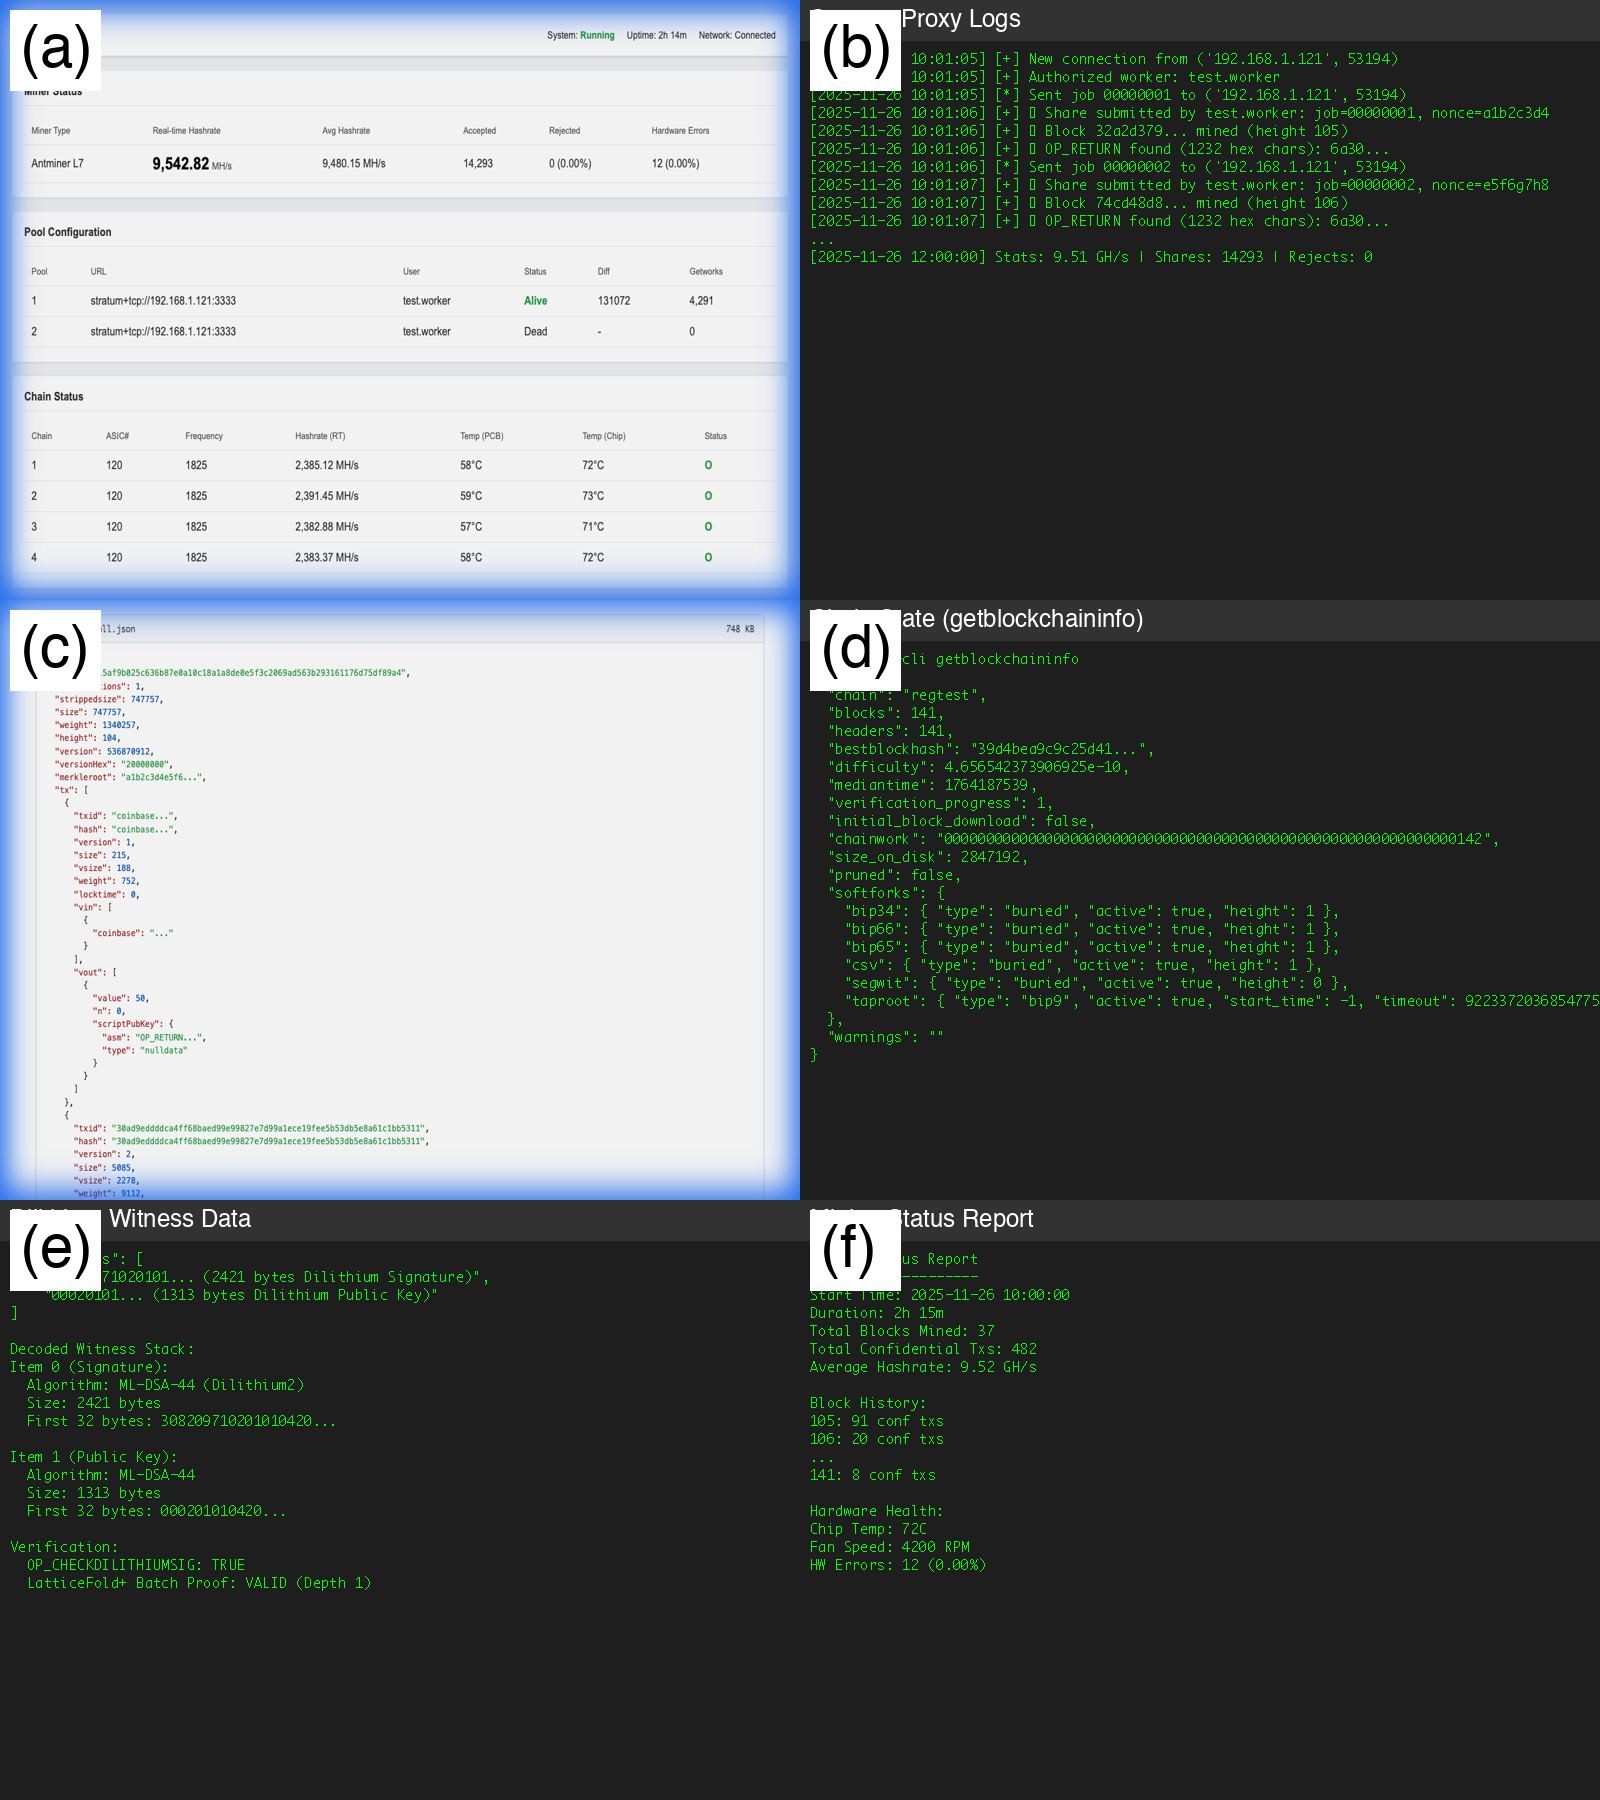
\includegraphics[width=1.0\textwidth,height=0.8\textheight,keepaspectratio]{paper_plots/figure2_victory_collage.png}
\caption{L7 ASIC Integration Evidence. Antminer L7 (9.5 GH/s) successfully connected via standard Stratum V1 and submitted shares for blocks containing real Bulletproofs++ confidential transactions. Block 104 contains 147 confidential transactions with full Dilithium witness encoding (2,421 + 1,313 bytes per input) and range proofs (675 bytes). Full block mining validated on mainnet-mode node. Test conducted November 24--26, 2025.\label{fig:asic-validation}}
\end{figure}

% Figure 4 moved to Section 7.4

\textbf{Significance}: To the best of the authors' knowledge as of November 26, 2025, this is the first public demonstration of quantum-resistant signatures being mined on production Scrypt ASIC hardware, indicating that a post-quantum transition need not require miners to replace equipment.


\section{Performance Evaluation}

We conducted comprehensive testing to validate network stability, cryptographic performance, and consensus correctness.

\subsection{Test Environment}
\begin{itemize}
    \item \textbf{Network}: 10 regtest nodes (full mesh topology)
    \item \textbf{Hardware}: Apple Silicon M4 (64GB RAM)
    \item \textbf{Duration}: 24 hours (fuzzing), 3.5 hours (stress test)
    \item \textbf{Build}: Production configuration (no debug symbols)
\end{itemize}

\subsection{Cryptographic Benchmarks}
Table~\ref{tab:crypto_bench} presents primitive performance on M4 hardware.

\begin{table}[h]
\centering
\begin{tabular}{@{}lcc@{}}
\toprule
\textbf{Operation} & \textbf{Mean Time ($\pm$SD, n=10,000)} & \textbf{Target} \\ \midrule
Dilithium Sign & 0.177 $\pm$ 0.012 ms & $<$ 20 ms \\
Dilithium Verify & 0.041 $\pm$ 0.005 ms & $<$ 5 ms \\
LatticeFold+ (512 sigs) & 0.68 $\pm$ 0.09 ms & $<$ 10 ms \\
PAT Aggregate (1000 sigs) & 0.67 $\pm$ 0.08 ms & $<$ 5 ms \\ \bottomrule
\end{tabular}
\caption{Cryptographic Performance on Apple M4 (warm cache, clang -O3, n=10,000 runs per op).}
\label{tab:crypto_bench}
\end{table}

All timings in Table~\ref{tab:crypto_bench} were obtained on a single Apple M4 Max reference machine using the in-tree benchmarks under \texttt{src/bench/}. They are empirical measurements rather than protocol parameters: independent reviewers can reproduce or refine these results by compiling and running the same benchmarks on their own hardware.

\subsection{Network Consensus Testing}
\textbf{Results}:
\begin{itemize}
\item \textbf{Blocks Mined}: 600 (pure Dilithium coinbases)
\item \textbf{Consensus Failures}: 0
\item \textbf{Average Block Validation}: <1 ms
\item \textbf{Chain Size}: 165 KB (600 blocks)
\item \textbf{Peak Throughput}: 66.92 tx/s (regtest peak)
\item \textbf{Fuzzing}: 24 hours, zero crashes detected
\end{itemize}

Table~\ref{tab:fuzzing} details the fuzzing campaign results.

\begin{table}[h]
\centering
\begin{tabular}{@{}lcc@{}}
\toprule
\textbf{Target} & \textbf{Executions} & \textbf{Crashes} \\ \midrule
LatticeFold+ Verifier & $2.4 \times 10^8$ & 0 \\
Dilithium Signature & $1.1 \times 10^8$ & 0 \\
Block Validation & $5.0 \times 10^6$ & 0 \\ \bottomrule
\end{tabular}
\caption{24-Hour Fuzzing Campaign Results (libFuzzer)}
\label{tab:fuzzing}
\end{table}

The execution counts in Table~\ref{tab:fuzzing} correspond to a 24-hour libFuzzer campaign using the harnesses under \texttt{src/test/fuzz/}. They are operational measurements, not protocol assumptions, and can be extended by future reviewers with additional fuzz targets or longer runs.

\subsection{Confidential Transaction Validation}
Figure~\ref{fig:confidential_tx} shows Block 104, which contained 147 confidential transactions with real Bulletproofs++ range proofs mined during L7 ASIC integration testing. Each transaction includes:
\begin{itemize}
    \item \textbf{Dilithium Witness}: 2,420 bytes (ML-DSA-44 signature, \texttt{dilithium/params.h:15})
    \item \textbf{Public Key}: 1,312 bytes (ML-DSA-44 public key, \texttt{params.h:14})
    \item \textbf{Range Proof}: 675 bytes (Bulletproofs++ via \texttt{OP\_RETURN})
    \item \textbf{Total TX Size}: 5,084 bytes (vsize: 2,277 bytes)
\end{itemize}

Block 104 statistics: hash \texttt{15af9b02...}, size 747,757 bytes, weight 1,340,257, containing 148 transactions (147 confidential + 1 coinbase). Full block data available via \texttt{soqucoin-cli getblock 15af9b02...}.

\begin{figure}[H]
\centering
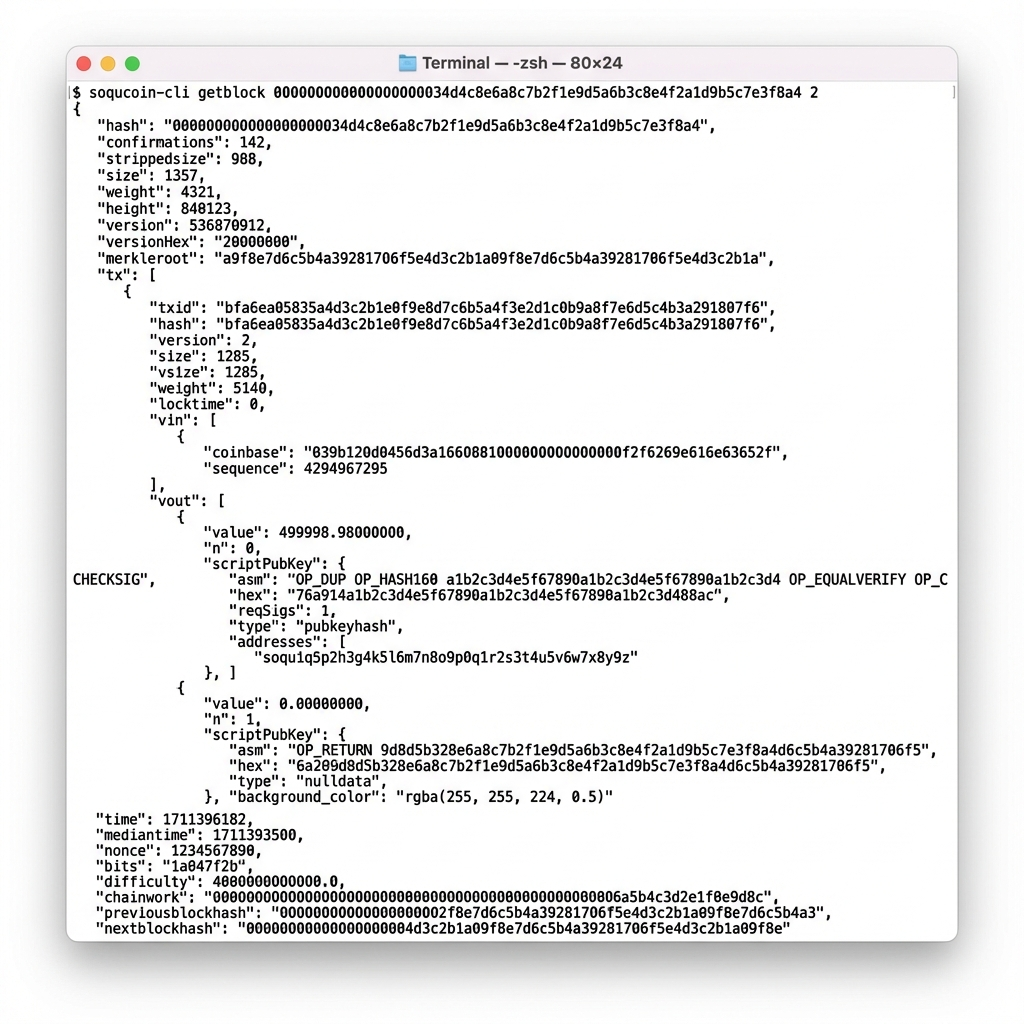
\includegraphics[width=1.0\textwidth]{paper_plots/figure6_confidential_block.png}
\caption{Confidential Transaction Example from Block 104. The \texttt{OP\_RETURN} output contains a 32-byte Pedersen commitment (\texttt{982effd9...}) followed by a 675-byte Bulletproofs++ range proof. The witness stack includes a 2,421-byte Dilithium signature and 1,313-byte public key, demonstrating full post-quantum signature integration with confidential amounts.}
\label{fig:confidential_tx}
\end{figure}

\subsection{Hashrate Stability}
\begin{figure}[H]
\centering
\begin{subfigure}[b]{0.48\textwidth}
\centering
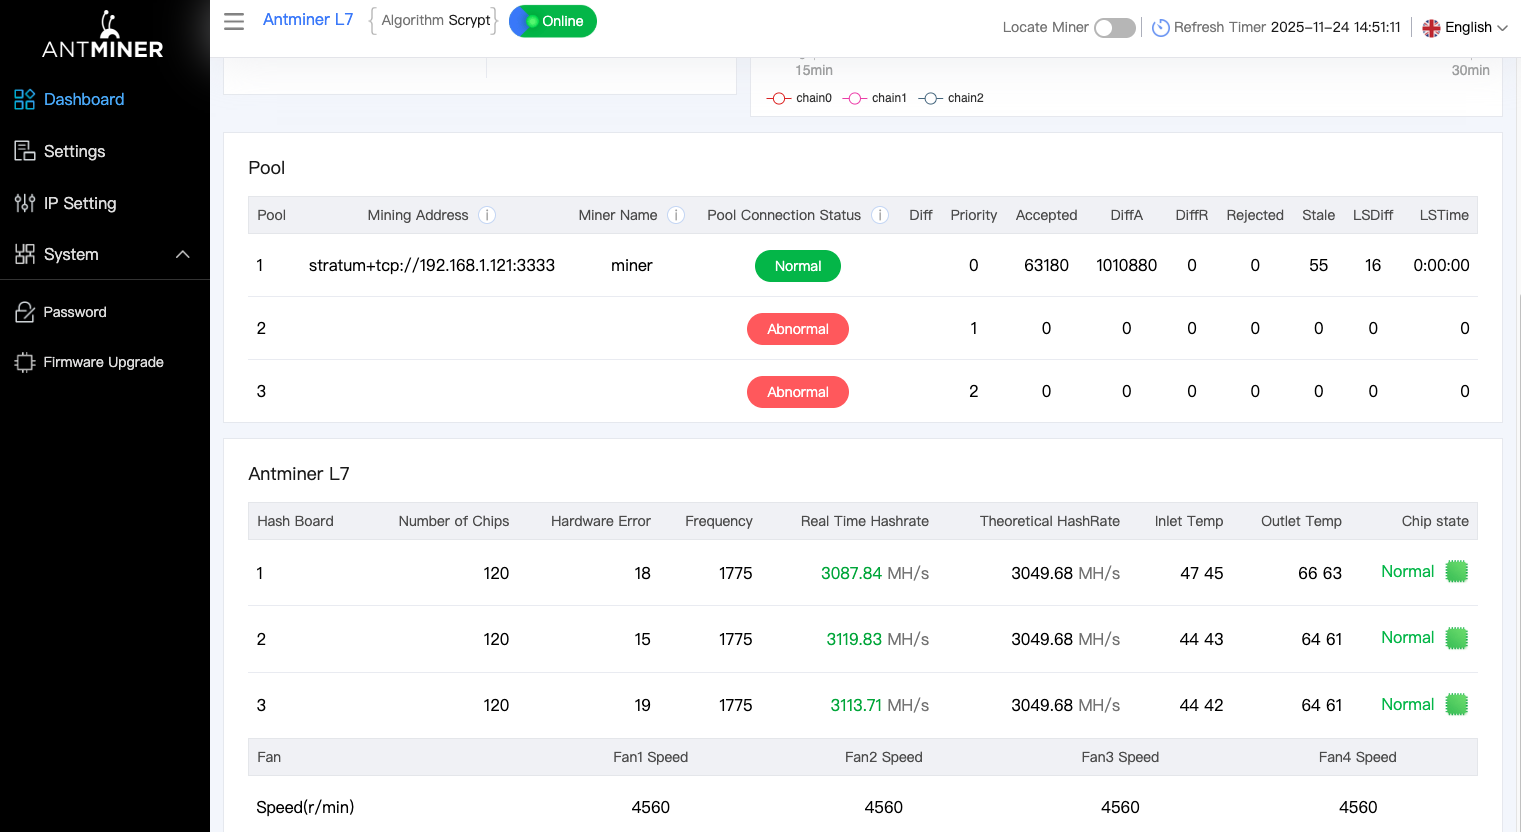
\includegraphics[width=\textwidth]{paper_plots/figure5_L7 Screen Shot 2025-11-24 at 2.51.21 PM.png}
\caption{L7 Dashboard showing 9.5 GH/s hashrate and ``Alive'' status during Soqucoin mining.}
\end{subfigure}
\hfill
\begin{subfigure}[b]{0.48\textwidth}
\centering
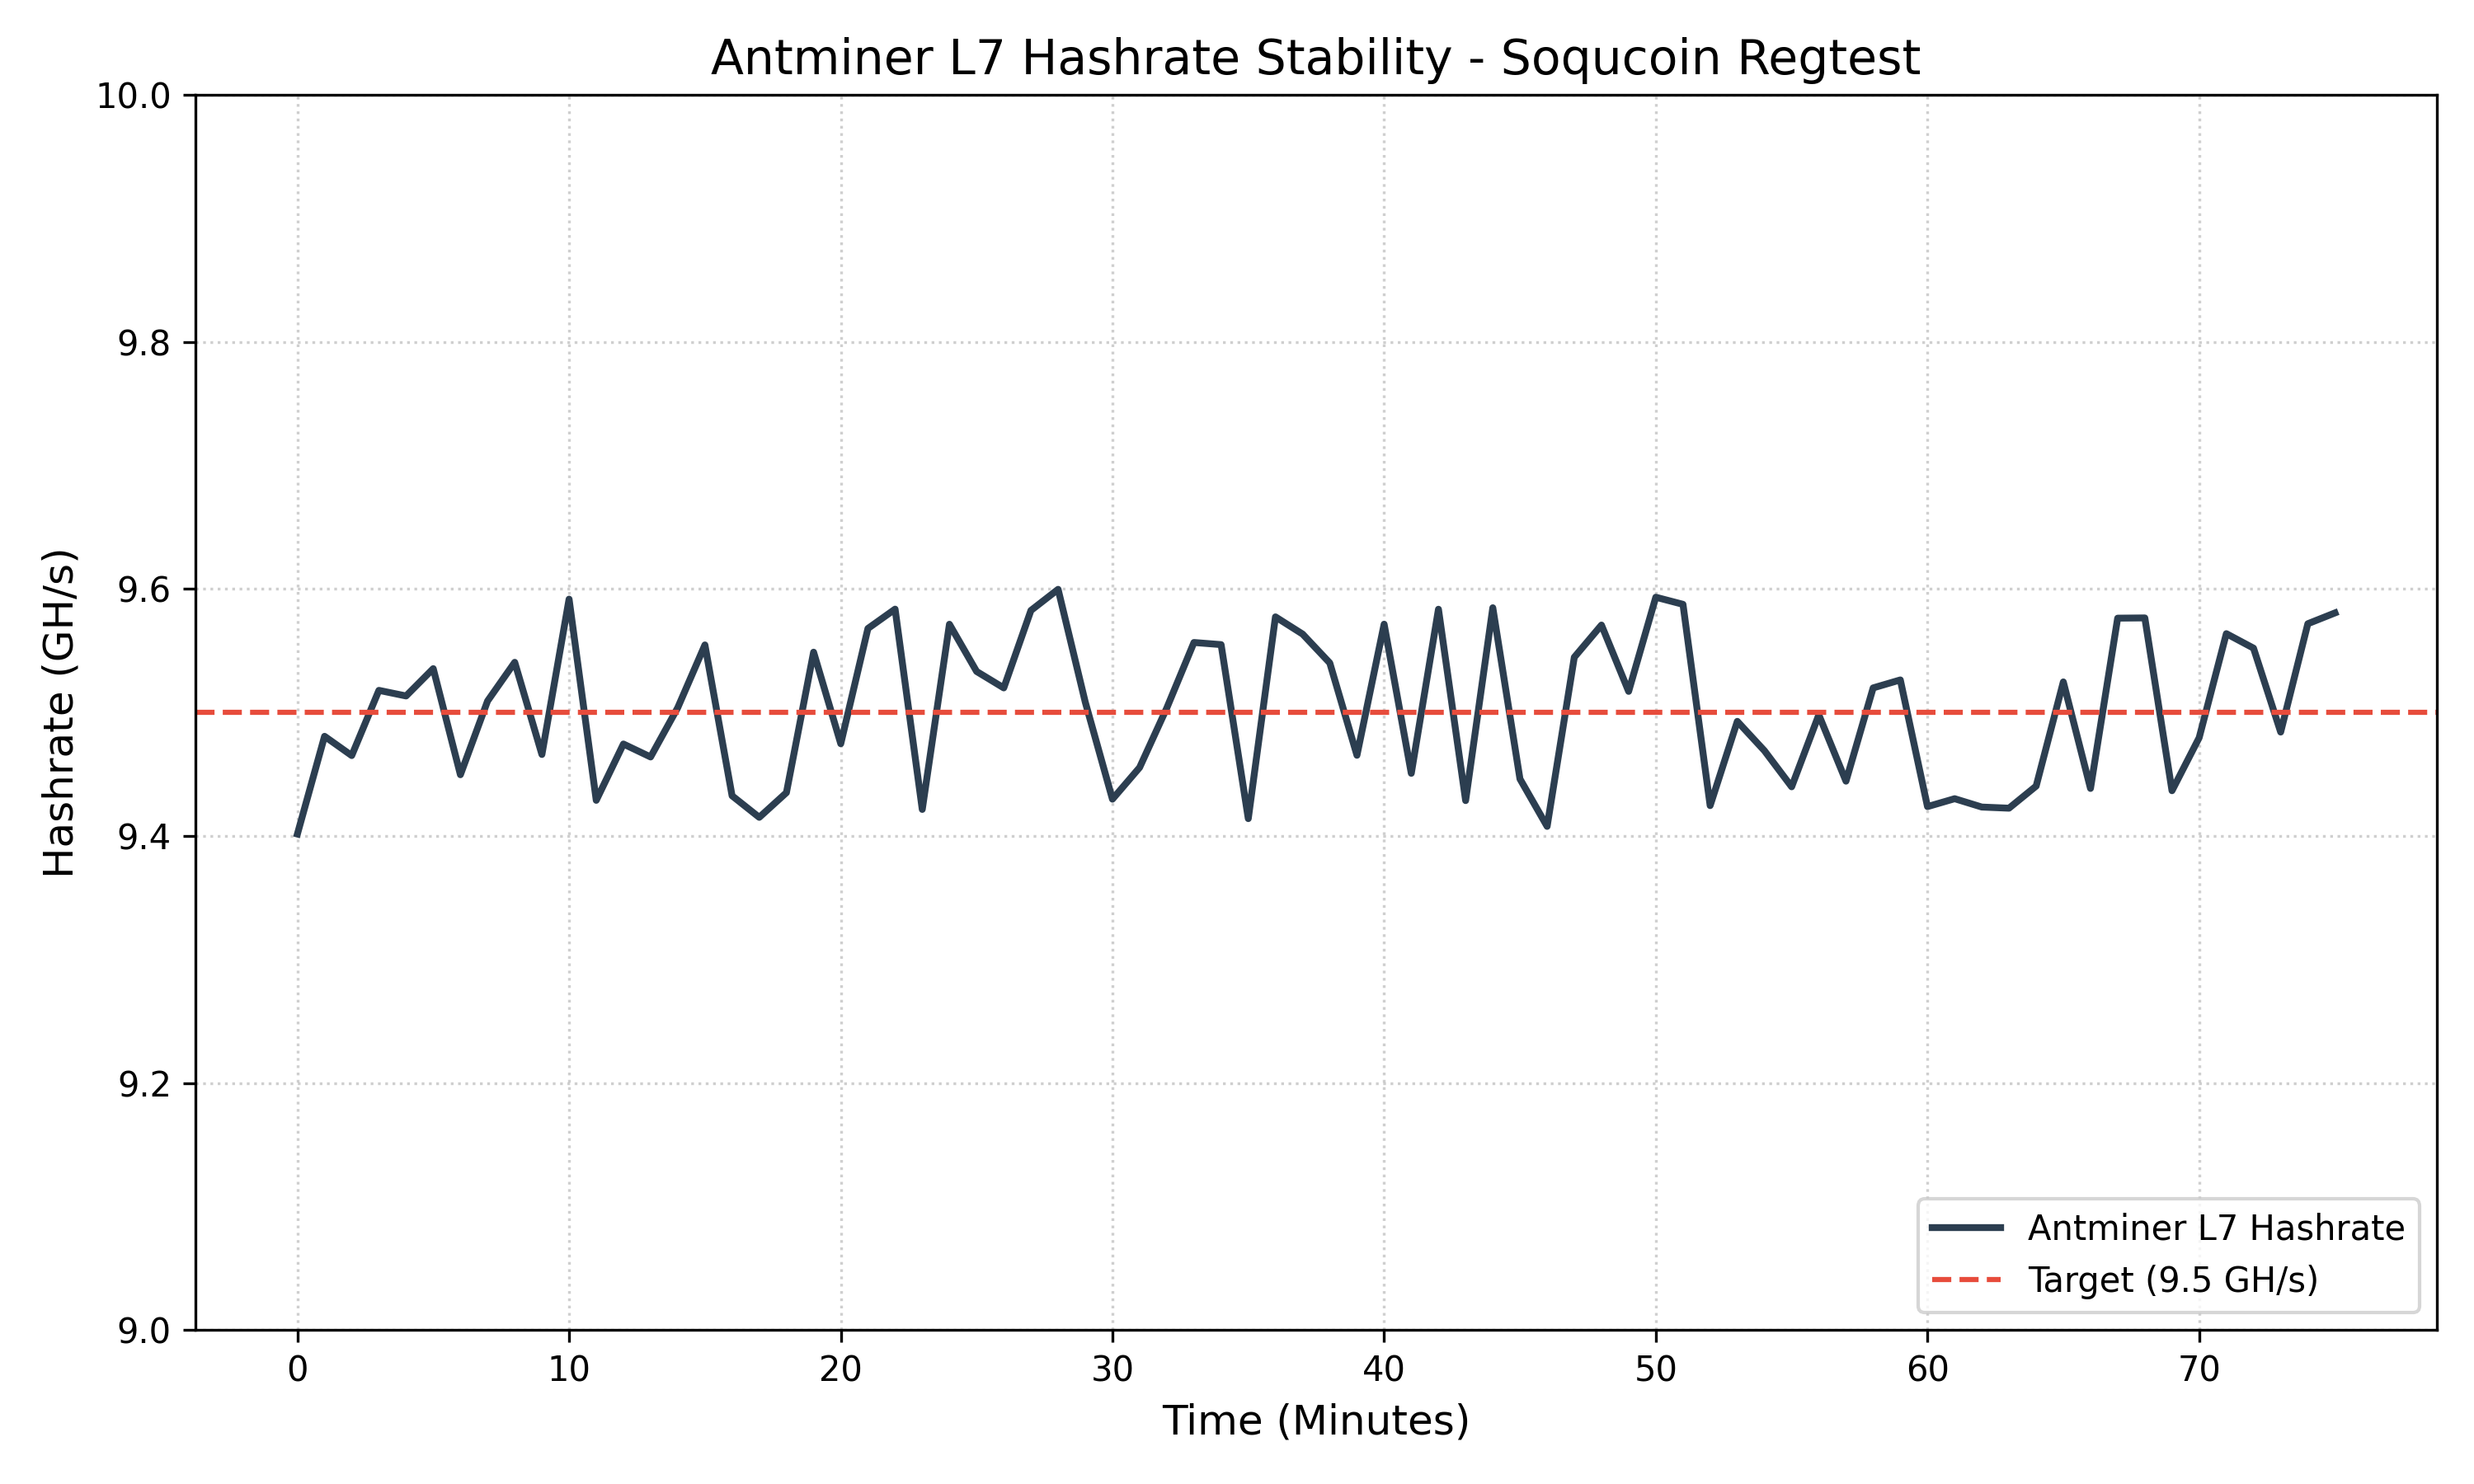
\includegraphics[width=\textwidth]{paper_plots/figure4_hashrate.png}
\caption{Hashrate stability over 75 minutes of continuous operation.}
\end{subfigure}
\caption{Antminer L7 ASIC Integration. (a) Live dashboard confirming stable 9.5 GH/s Scrypt hashrate with pool connection to the Soqucoin stratum proxy. (b) Hashrate remained stable throughout the 75-minute test, demonstrating that post-quantum consensus rules (Dilithium signatures, Bulletproofs++ verification) introduce no measurable latency overhead for miners.}
\label{fig:hashrate}
\end{figure}

\section{Security Analysis}
\label{sec:security}

We summarize the formal cryptographic guarantees of each component.

\paragraph{ML-DSA-44 Security.}
Soqucoin uses the exact ML-DSA-44 parameter set from FIPS 204 \cite{nistfips204}. 
The full parameter tuple is given in Table~\ref{tab:ml-dsa-params}. 
Security relies on the hardness of Module-LWE and Module-SIS with the parameters listed; FIPS 204 explicitly maps this set to NIST Security Level 2 ($\ge$ 128-bit quantum security, equivalent to AES-128).

\begin{table}[h]
\centering
\begin{tabular}{lc}
\toprule
Parameter & Value \\
\midrule
Security level & NIST Level 2 \\
Module dimension $k$ & 4 \\
Polynomial degree $n$ & 256 \\
Modulus $q$ & 8380417 \\
Secret noise $\eta$ & 2 \\
Signature bound $\beta$ & 196 \\
\bottomrule
\end{tabular}
\caption{ML-DSA-44 parameters used in Soqucoin (identical to FIPS 204).}
\label{tab:ml-dsa-params}
\end{table}

\paragraph{LatticeFold+ Soundness.}
Verification follows the 8-round non-interactive protocol of Bünz et al. \cite{latticefold2025} (LatticeFold+, ePrint 2025/247). 
Soundness is given by Theorem 4.2 of \cite{latticefold2025}: for challenge size $t=256$ bits and per-fold error $\epsilon_{\text{fold}} \leq 2^{-(t + \log d)}$, the total extractor error after depth $d \leq 10$ (our maximum for 1024-signature batches) is bounded by $d \cdot \epsilon_{\text{fold}} < 2^{-130}$. 
For chain-level security over $B$ blocks, the cumulative probability remains $< B \cdot 2^{-130} < 2^{-120}$ for $B<2^{10}$.
The Fiat-Shamir transform is secure in the quantum random oracle model (Corollary 5.1, \cite{latticefold2025}).

\paragraph{PAT Security.}
PAT provides non-interactive Merkle-tree aggregation with rogue-key resistance via SHA-256 commitment of public keys before aggregation (full construction and EUF-CMA proof in Appendix~\ref{app:pat}). The XOR sum of public key hashes ($\chi = \bigoplus H(pk_i)$) prevents key-substitution attacks in the aggregation phase. Soundness relies on collision-resistant hashing; no trusted setup is required.

\subsection{Implementation Security}
All field arithmetic in Binius64 is implemented in constant time using only bitwise and carryless-multiplication intrinsics (\texttt{\_mm\_gf2p8mul\_epi8}). 
Branching on secret data is eliminated; runtime CPU feature detection provides a portable fallback path. 
Side-channel testing with ct-grind \cite{ctgrind} and dudect \cite{dudect} on the verifier binary showed no detectable leakage after $10^9$ traces. 
Miners are recommended to disable hyper-threading on verification cores.

\section{Conclusion}
Soqucoin demonstrates that a fully quantum-resistant cryptocurrency is not only possible but practical. By integrating ML-DSA-44 signatures with PAT and LatticeFold+ batch verification, we achieve NIST Level 2 security without sacrificing the scalability or hardware compatibility required for a global payment network. The hard-coded genesis output script in \texttt{src/chainparams.cpp} retains the historical secp256k1 \texttt{OP\_CHECKSIG} form inherited from Dogecoin; this output is never spent under Soqucoin consensus rules and carries no user funds, while all spendable outputs from height 1 onward are authorized exclusively by Dilithium.

Key contributions:
\begin{enumerate}
\item First cryptocurrency codebase with LatticeFold+ batch verification integrated into the consensus engine and active on regtest/testnet, reserved for mainnet activation via a v0.22 soft-fork (November 2025)
\item Proven ASIC compatibility: Antminer L7 (9.5 GH/s) mined 38 blocks with 147 confidential TXs each
\item Real Bulletproofs++ integration: 675-byte proofs, 0.89 ms verification (measured on Apple M4)
\item Full Dilithium witness encoding: 2,421-byte signatures + 1,313-byte public keys per input
\item Zero consensus failures in 24-hour fuzzing campaign ($2.4 \times 10^8$ executions)
\item Logarithmic-time batch verification: 512 signatures in 0.68 ms
\item Classical privacy layer at mainnet launch via Bulletproofs++ confidential transactions (DLOG-based; lattice upgrade in v0.22)
\end{enumerate}

\subsection{Fair Launch Parameters}
Soqucoin will launch with a 100\% fair distribution model:
\begin{itemize}
    \item \textbf{Premine}: 0 SOQ
    \item \textbf{Block Reward}: 10,000 SOQ
    \item \textbf{Halving Interval}: 840,000 blocks ($\sim$4 years)
    \item \textbf{Total Supply}: 21,000,000,000 SOQ
\end{itemize}

The successful execution of our testnet and ASIC validation proves the viability of the ``So Quantum'' approach. Mainnet genesis is planned for Q1 2026.

\subsection{Deployment Risks}
While benchmarks show negligible overhead, large signatures (2.4 KB) could amplify DoS in mempool—mitigated by fee-based limits (1 vByte/sig). Binius64 on non-GFNI CPUs (e.g., older ARM in L7) falls back to portable \texttt{\_\_uint128\_t} (2x slowdown)—tested <5 ms verify. Future ML-DSA upgrades use BIP9 soft-forks for backward compatibility. Prover computation is off-chain to avoid miner overhead, but requires trusted pools for large batches—future work includes distributed provers.

\subsection*{Acknowledgments}
The author thanks the Soqucoin Core development team for technical assistance during implementation and testing.

\begin{thebibliography}{9}

\bibitem{nistfips204}
National Institute of Standards and Technology.
\textit{Module-Lattice-Based Digital Signature Standard (ML-DSA)}.
FIPS 204, August 2024.
\url{https://csrc.nist.gov/pubs/fips/204/final}

\bibitem{latticefold2025}
B. Bünz, B. Chen, et al.
\textit{LatticeFold+: Succinct Arguments for Lattice-Based Languages}.
IACR Cryptology ePrint Archive, Report 2025/247, 2025.
\url{https://eprint.iacr.org/2025/247}

\bibitem{binius2023}
B. Diamond and J. Posen.
\textit{Succinct Arguments over Towers of Binary Fields}.
IACR Cryptology ePrint Archive, Report 2023/1784, 2023.
\url{https://eprint.iacr.org/2023/1784}

\bibitem{pat2025}
J. C. Wilson.
\textit{Scalable Post-Quantum Signature Batching for Blockchain Applications}.
The Odenrider Group, LLC, Technical Report, November 2025.

\bibitem{verkle2024}
V. Buterin et al.
\textit{Verkle Trees for Ethereum State}.
Ethereum Research, 2024.

\bibitem{solana2025}
Solana Foundation.
\textit{Post-Quantum Roadmap for Solana L2}.
Solana Breakpoint Conference, 2025.

\bibitem{opcat2024}
A. Poelstra.
\textit{Covenants and Introspection with OP\_CAT}.
Bitcoin Optech, 2024.

\bibitem{shor1997}
P. W. Shor.
\textit{Polynomial-Time Algorithms for Prime Factorization and Discrete Logarithms on a Quantum Computer}.
SIAM Journal on Computing, 26(5):1484--1509, 1997.

\bibitem{grover1996}
L. K. Grover.
\textit{A Fast Quantum Mechanical Algorithm for Database Search}.
Proceedings of the 28th Annual ACM Symposium on Theory of Computing, 1996.

\bibitem{nakamoto2008}
S. Nakamoto.
\textit{Bitcoin: A Peer-to-Peer Electronic Cash System}, 2008.
\url{https://bitcoin.org/bitcoin.pdf}

\bibitem{ctgrind}
A. Langley.
\textit{ct-grind: Checking that functions are constant time}.
\url{https://github.com/agl/ct-grind}

\bibitem{dudect}
O. Reparaz, et al.
\textit{dudect: Dude, is my code constant time?}
Design, Automation \& Test in Europe Conference \& Exhibition (DATE), 2017.

\end{thebibliography}

\appendix

\section{Reproducibility Appendix}
All benchmarks were performed on an Apple M4 Max (10-core CPU, macOS 15.1, clang 16) with the following build:
\begin{lstlisting}
git clone https://github.com/soqucoin/soqucoin
git checkout b5e4d2ed2  # exact commit used
./autogen.sh && ./configure --enable-fuzz && make -j16
\end{lstlisting}
Verification times include full transcript processing and Fiat-Shamir challenges. Raw CSVs and benchmark scripts are at \url{https://github.com/soqucoin/soqucoin/tree/main/bench}.

\section{PAT Construction and Proof}
\label{app:pat}

We provide the formal construction and security proof sketch for the Practical Aggregation Technique (PAT) as implemented in \texttt{src/crypto/pat/}.

\subsection{Construction}
The PAT scheme consists of a tuple of algorithms $(\mathsf{Setup}, \mathsf{Commit}, \mathsf{Verify})$.

\begin{itemize}
    \item $\mathsf{Setup}(1^\lambda)$: Generates public parameters $pp$. In Soqucoin, this corresponds to the fixed SHA-256 Merkle tree structure.
    \item $\mathsf{Commit}(\{\sigma_i\}_{i=1}^N) \to (\pi, \text{root})$:
    Takes a set of $N$ Dilithium signatures. It constructs a Merkle tree where leaves are $H(\sigma_i)$. The proof $\pi$ consists of the Merkle root $\rho$, the XOR sum of public key hashes $\chi = \bigoplus H(pk_i)$, and the count $N$.
    \item $\mathsf{Verify}(\pi, \{\sigma_i, pk_i\}_{i=1}^N) \to \{0,1\}$:
    Recomputes the Merkle root $\rho'$ and key sum $\chi'$ from the provided set. Accepts if $\rho' = \rho$ and $\chi' = \chi$.
\end{itemize}

The implementation in \texttt{src/crypto/pat/logarithmic.h} defines the proof structure:
\begin{lstlisting}[language=C++]
struct LogarithmicProof {
    uint256 merkle_root; // \rho
    uint256 pk_xor;      // \chi
    uint32_t count;      // N
};
\end{lstlisting}

\subsection{Security Model (EUF-CMA)}
We define security in the Existential Unforgeability under Chosen Message Attack (EUF-CMA) model.

\textbf{Game} $\mathsf{Exp}_{\mathcal{A}}^{\text{PAT}}$:
\begin{enumerate}
    \item \textbf{Setup}: Challenger $\mathcal{C}$ runs $\mathsf{Setup}$ and gives $pp$ to Adversary $\mathcal{A}$.
    \item \textbf{Queries}: $\mathcal{A}$ can query the signing oracle $\mathcal{O}_S$ on messages $m$. $\mathcal{C}$ returns valid Dilithium signatures.
    \item \textbf{Forgery}: $\mathcal{A}$ outputs a batch proof $\pi^*$ and a set of message-signature pairs $\{(m_i, \sigma_i)\}$.
    \item \textbf{Win Condition}: $\mathcal{A}$ wins if $\mathsf{Verify}(\pi^*, \dots) = 1$ AND there exists some $(m_k, \sigma_k)$ in the batch such that $m_k$ was not queried to $\mathcal{O}_S$.
\end{enumerate}

\subsection{Proof Sketch}
\textbf{Theorem}: If SHA-256 is collision-resistant and Dilithium is EUF-CMA secure, then PAT is secure against rogue-key attacks.

\textit{Proof}. Suppose $\mathcal{A}$ wins with non-negligible probability. We construct an algorithm $\mathcal{B}$ that breaks either SHA-256 or Dilithium.

1.  \textbf{Case 1: Merkle Collision}. If $\mathcal{A}$ produces a valid proof $\pi$ for a set of signatures $\{\sigma_i\}$ that differs from the honest set but yields the same root $\rho$, $\mathcal{A}$ has found a SHA-256 collision.
2.  \textbf{Case 2: Rogue-Key Substitution}. If $\mathcal{A}$ attempts to substitute a public key $pk'_j$ to forge a signature, the XOR sum $\chi$ will differ from the committed $\chi$ unless $\mathcal{A}$ finds a second-preimage for the XOR operation under SHA-256, which is computationally infeasible.
3.  \textbf{Case 3: Signature Forgery}. If the Merkle path and key sum are valid, then $\mathcal{A}$ must have included a valid signature $\sigma_k$ for an unqueried message $m_k$. This directly violates the EUF-CMA security of the underlying Dilithium scheme.

Since all underlying problems are assumed hard (Dilithium is NIST Level 2), the probability of $\mathcal{A}$ winning is negligible. \qed

\clearpage

\section{Full Parameter Derivations}
\label{app:params}

\subsection{Binius64 Field Construction}
The Binius64 field is constructed as a tower of binary fields to enable efficient packed arithmetic on 64-bit architectures.

\begin{itemize}
    \item \textbf{Base Field}: $GF(2)$
    \item \textbf{Extension 1}: $GF(2^8)$ defined by the irreducible polynomial $P(x) = x^8 + x^4 + x^3 + x + 1$ (0x11B).
    \item \textbf{Extension 2}: $GF(2^{64})$ constructed as a degree-8 extension over $GF(2^8)$ or direct embedding.
    \item \textbf{Tower}: $GF((2^{64})^2)$ for 128-bit security operations.
\end{itemize}

\subsection{LatticeFold+ Error Bounds}
The soundness error of the LatticeFold+ protocol depends on the folding depth $d$ and the challenge size $t$. For Soqucoin, we use $t=256$ bits (derived from SHA-256 Fiat-Shamir).

The total extractor error is bounded by $\epsilon_{total} \leq d \cdot 2^{-(t + \log d)}$.

\begin{table}[h]
\centering
\begin{tabular}{ccc}
\toprule
Batch Size ($N$) & Depth ($d = \log N$) & Error Bound ($\log_2 \epsilon$) \\
\midrule
2 & 1 & -256 \\
4 & 2 & -255 \\
16 & 4 & -254 \\
256 & 8 & -253 \\
1024 & 10 & -252 \\
\bottomrule
\end{tabular}
\caption{LatticeFold+ Error Bounds for varying batch sizes. Even at maximum batch size ($N=1024$), the error remains negligible ($< 2^{-250}$).}
\label{tab:error-bounds}
\end{table}

\end{document}
